\section{Werbung, HTML-Wanzen und Social Media}
Die auf vielen Websites eingeblendete \textbf{Werbung }wird von wenigen Servern bereitgestellt. Diese nutzen h�ufig (eigentlich immer) die damit gegebenen M�glichkeiten, das Surfverhalten �ber viele Websites hinweg zu erfassen. Mit Hilfe von listen- und musterbasiert Filtern kann der Zugriff auf Werbung sowie die von diesen Servern genutzten Cookies unterbunden werden.\\

Hinweis: Viele Angebote im Web werden �ber Werbung finanziert, da die Nutzer meist nicht bereit sind, f�r diese Angebote zu bezahlen. Die Redaktion von Heise.de hat ein kurzes Statement\footnote{ \href{http://www.heise.de/Adblocker-auf-heise-online-1164703.html}{http://www.heise.de/Adblocker-auf-heise-online-1164703.html}} zu Werbung auf Heise online ver�ffentlicht und erkl�rt, wie sie einzelne Webangebote durch Freigaben im Werbeblocker unterst�tzen k�nnen.\\

Bei \textbf{HTML-Wanzen} (sogenannten Webbugs) handelt es sich um 1x1-Pixel gro�e transparente Bildchen, welche in den HTML-Code einer Webseite oder einer E-Mail eingebettet werden. Sie sind f�r den Nutzer unsichtbar und werden beim Betrachten einer Webseite oder beim �ffnen der E-Mail von einem externen Server geladen und erm�glichen es dem Betreiber des Servers, das Surfverhalten website�bergreifend zu verfolgen.\\

Hinweis: das System METIS\footnote{ \href{http://www.vgwort.de/metis.php}{http://www.vgwort.de/metis.php}} der VG Wort verwendet HTML-Wanzen, um die Besucher von Online-Angeboten zu z�hlen und anhand der Ergebnisse Tantiemen an Autoren auszuzahlen.\\

Facebook und andere Sociale Netze verwenden sogenannte \textbf{Like Buttons}, um Daten zu sammeln. Die Verwendung der Like Buttons ist nach Ansicht von Thilo Weichert (ULD) nicht mit deutschen Datenschutzrecht vereinbar. Deutsche Webseitenbetreiber sind aufgefordert, die Facebook Buttons von ihren Seiten zu entfernen\footnote{ \href{https://www.datenschutzzentrum.de/facebook/}{https://www.datenschutzzentrum.de/facebook}}. Mit dem Aufruf einer Webseite, die den Like Button enth�lt, werden Daten an Facebook �bertragen und dort ausgewertet.\\

Forscher der Universit�t Cambridge (Gro�britannien) konnten im Rahmen einer Untersuchung durch Auswertung der Klicks auf Facebook Like Buttons die sexuelle Orientierung und politische Einstellung der Teilnehmer vorhersagen\footnote{ \href{http://heise.de/-1820638}{http://heise.de/-1820638}}. Man verr�t mit einem Klick auf einen Like Button m�glicherweise Informationen, die man nicht im Netz ver�ffentlichen m�chte. 

\subsection{Tracking-Filter f�r Firefox}
Es gibt mehrere Add-ons f�r Firefox, die Werbung und Trackingelemente blockieren. Das Center for Internet and Society der Stanford Law School hat in einer Analyse vom September 2011 einige L�sungen verglichen \footnote{ \href{https://cyberlaw.stanford.edu/node/6730}{https://cyberlaw.stanford.edu/node/6730}}. Die Ergebnisse in Bild \ref{abb:trackingfilter} zeigen: keine L�sung ist perfekt.\\

\begin{figure}[htb]
\begin{center}
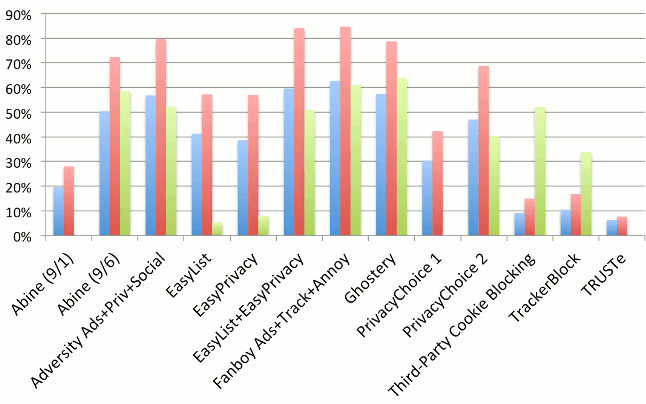
\includegraphics[scale=1.0]{../screenshots/tracking-blocker.png}
\caption{Effektivit�t verschiedener Tracking-Filter}
\label{abb:trackingfilter}
\end{center}
\end{figure}

Aufgrund der Flexibilit�t bei der Einbindung verschiedener Filterlisten empfehle ich \textit{AdBlock Plus}. Mit den Easylist Filterlisten erreichten das Add-on bei dem Test mit die besten Ergebnisse. Die Listen werden st�ndig weiterentwickelt. Es gibt als Zusatz eine spezielle Filterliste f�r deutsche Webseiten.\\

Zus�tzlich zur den Blocklisten\textit{ EasyList+Germany} und \textit{EasyPrivacy} sollte man noch eine Liste abonnieren, die die Social Media Buttons blockiert, z.B. \textit{SocialMediaBlock} von MontzA.\\

\textit{FanBoy} arbeitet seit 2010 mit EasyList zusammen, daher die �hnlich guten Ergebnisse. \textit{Ghostery} schneidet im Test auch gut ab und wird oft empfohlen. Es gibt aber immer wieder Probleme mit Ghostery auf einigen Webseiten, da das Add-on kein Whitelisting kennt. Au�erdem arbeitet es mit einer festen Blockliste, die nicht flexibel erweitert oder kombiniert werden kann. 